\documentclass{standalone}
%\pagenumbering{gobble}


%%%%%%%%%%%%%%%%%%%%%%%%%%%%%%%%%%%%%%%%%%%%
% collision cylinder
%
%%%%%%%%%%%%%%%%%%%%%%%%%%%%%%%%%%%%%%%%%%%%


\usepackage{tikz,xcolor}
\usetikzlibrary{arrows,snakes}

\tikzset{
	partial ellipse/.style args={#1:#2:#3}{insert path={+ (#1:#3) arc (#1:#2:#3)}}
	}

\begin{document}


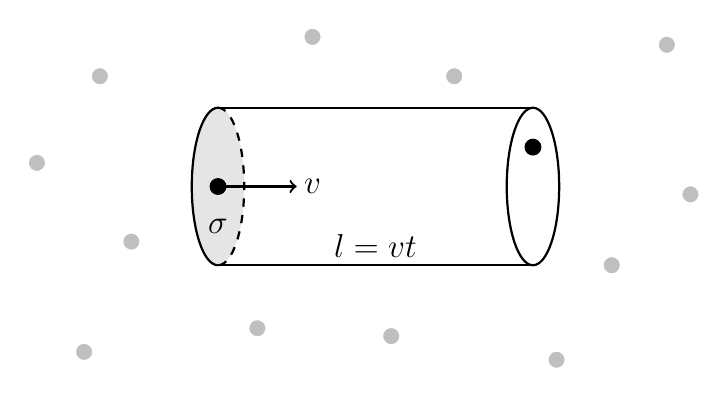
\begin{tikzpicture}[scale=1.0, font=\sffamily]

	% ellipse with dotted back side
	\draw[thick, fill=gray!20] (3,0) [partial ellipse=-90:90:-0.333 and 1];
	\draw[thick, dashed, fill=gray!20] (3,0) [partial ellipse=90:-90:0.333 and 1];
	% end of cylinder
	\draw[thick] (7,0) ellipse (0.333 and 1);
	% side of cylinder
	\draw[thick] (3,1) -- (7,1);
	\draw[thick] (3,-1) -- (7,-1);
	% annotation
	\node[align=center] at (4.2,0) {\large $v$};
	\node[align=center] at (5.0,-0.75) {\large $l=vt$};
	\node[align=center] at (3.0,-0.5) {\large $\sigma$};

	% collider
	\draw[fill] (3,0) circle (0.1);
	\draw[thick, ->] (3,0) -- (4,0);

	% target
	\draw[fill] (7,0.5) circle (0.1);

	% background
	%\draw[color=white, fill=gray!50] (0,-1.2) circle (0.11);
	\draw[color=white, fill=gray!50] (0.7,0.3) circle (0.11);
	\draw[color=white, fill=gray!50] (1.3,-2.1) circle (0.11);
	\draw[color=white, fill=gray!50] (1.5,1.4) circle (0.11);
	\draw[color=white, fill=gray!50] (1.9,-0.7) circle (0.11);
	\draw[color=white, fill=gray!50] (3.5,-1.8) circle (0.11);
	\draw[color=white, fill=gray!50] (4.2,1.9) circle (0.11);
	\draw[color=white, fill=gray!50] (5.2,-1.9) circle (0.11);
	\draw[color=white, fill=gray!50] (6.0,1.4) circle (0.11);
	\draw[color=white, fill=gray!50] (7.3,-2.2) circle (0.11);
	\draw[color=white, fill=gray!50] (8,-1) circle (0.11);
	\draw[color=white, fill=gray!50] (8.7,1.8) circle (0.11);
	\draw[color=white, fill=gray!50] (9,-0.1) circle (0.11);

\end{tikzpicture}

\end{document} 
